\documentclass[13pt]{beamer}

\usepackage{url}
\usepackage{graphicx}

\usefonttheme{structurebold}
\setbeamercolor{background canvas}{bg=black}
\setbeamercolor{normal text}{fg=white}
\setbeamercolor{structure}{fg=white}
\setbeamertemplate{navigation symbols}{}

\title{Uncommon things we do}
\author{
        Chris Lamb \\
        \vskip 6mm
        \tiny{\url{chris@chris-lamb.co.uk}}
}
\date{}

\begin{document}

\centering

\frame{
	\titlepage
    
\includegraphics[width=15mm]{img/thread.png}
}

\frame {}

\frame {
    Uncommon things

    \vskip 1em

    \begin{itemize}
        \item "Oh that's interesting"
        \item Uncommon vs. should be common
    \end{itemize}
}

\frame {}

\frame {
    Thread.com history redux

    \vskip 1em

    \begin{itemize}
        \item Playfire.com, social networking site for gamers
        \begin{itemize}
            \item Zero to 1.5 million members
            \item Automatic tracking Xbox 360, PlayStation 3 and PC gameplay in March 2011
            \item Huge site, massive data, scaling fun
            \item Released lots of free software components
        \end{itemize}
        \item Acquired May 2012
        \item YCombinator S12
    \end{itemize}
}

\frame {}

\frame {
    1/4: Pulse
}

\frame {
    Pulse channel
    \vskip 1em
    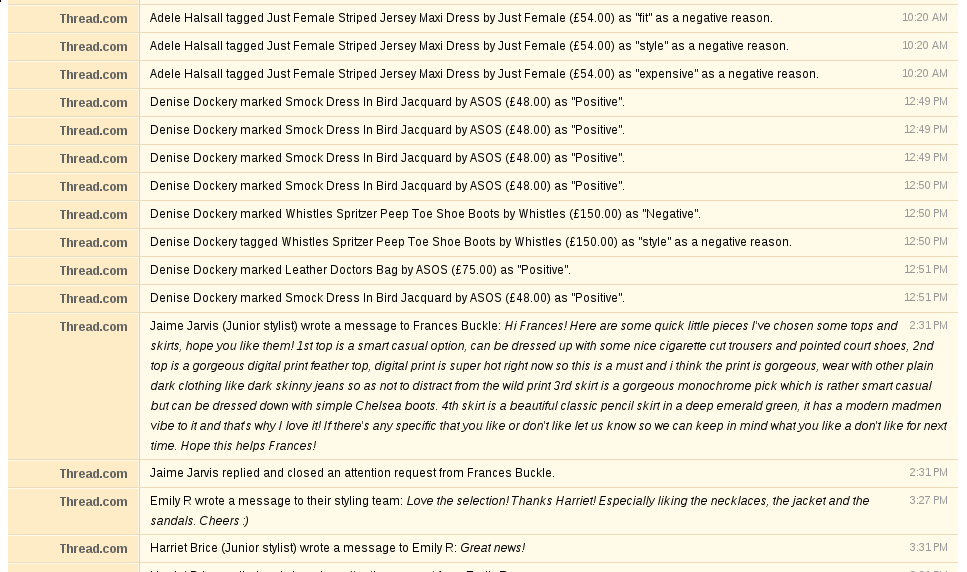
\includegraphics[width=100mm]{img/pulse.png}
}

\frame {
    \begin{itemize}
        \item For visibility, not auditing
        \item We put important events in our main channel, everything else in "Pulse"
        \item History for free
        \item Any chat technology can work
        \item \url{https://github.com/thread/django-hipchat}
    \end{itemize}
}

\frame {
    History
    \vskip 1em
    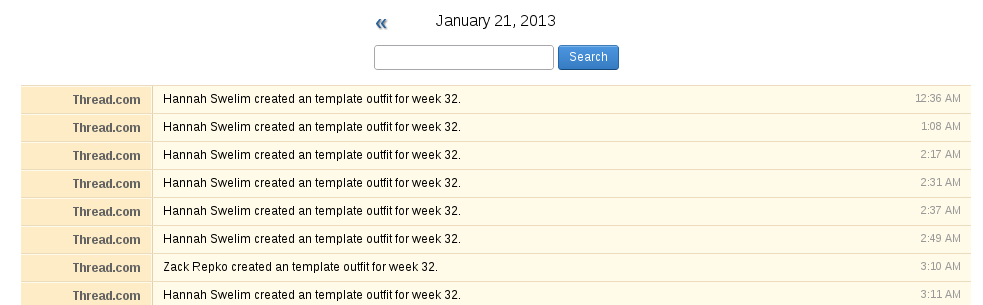
\includegraphics[width=100mm]{img/pulse-history.png}
}

\frame {
    2/4: Deploying using Debian packages
}

\frame {
    Playfire.com old {\em old} build process
    \vskip 1em
    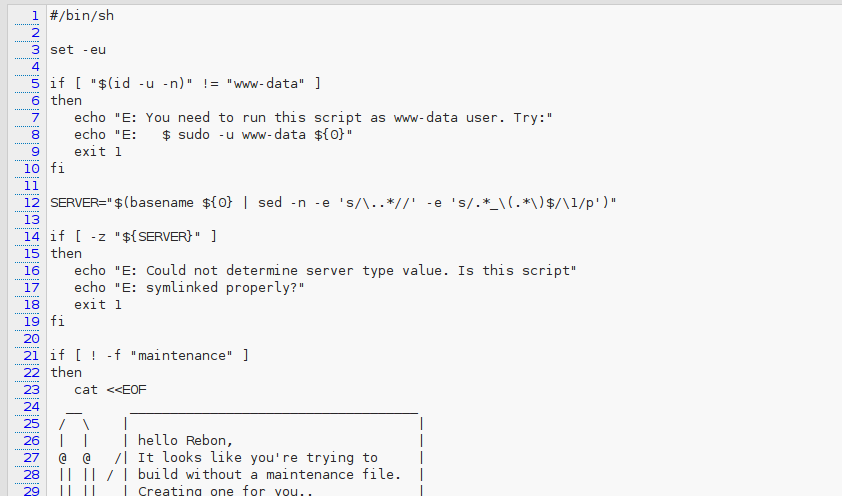
\includegraphics[width=100mm]{img/build-script.png}
}

\frame {
    Outline

    \vskip 1em

    \begin{itemize}
        \item Build .deb
        \item rsync to target hosts
        \item Install with {\tt dpkg -i}
    \end{itemize}
}

\frame {
    Advantages
    
    \vskip 1em

    \begin{itemize}
        \item Can happily work with system packages
        \item Many tasks already done for you very well (debhelper)
        \item Easy to make modular system
        \item Can change a machine's purpose cleanly without reimaging
        \item Can distribute packages centrally with APT
        \item Can scale up to very compl. (APT/{\tt dak}/{\tt mini-dinstall})
    \end{itemize}
}

\frame {
    Disadvantages

    \vskip 1em

    \begin{itemize}
        \item Requires distribution-specific knowledge
        \item Inherits all Debian legacy packaging quirks
        \item Installing standalone packages with {\tt dpkg} problematic
    \end{itemize}
}

\frame {
    Example Thread.com deployment
    \vskip 1em
    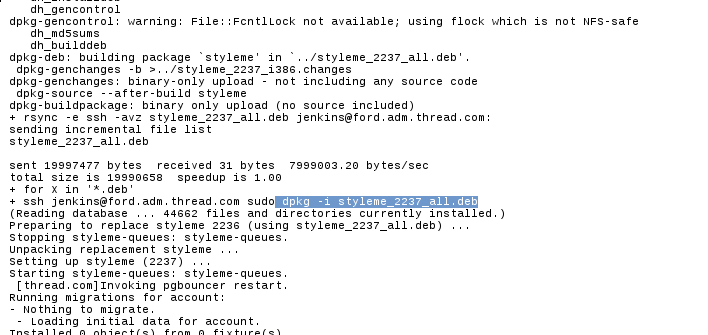
\includegraphics[width=100mm]{img/debian-deploy.png}
}

\frame {
    \tt{debian/control}
    \vskip 1em
    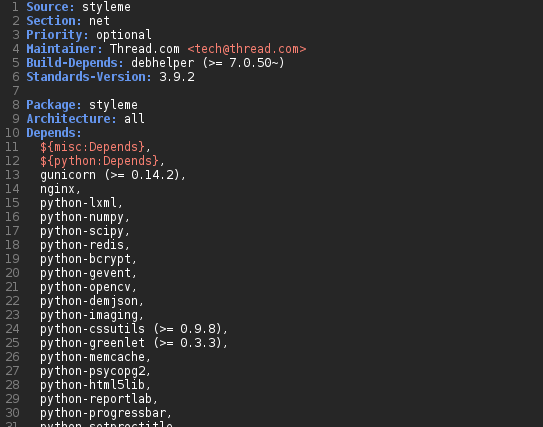
\includegraphics[width=100mm]{img/debian-control.png}
}

\frame {
    \tt{debian/postinst}
    \vskip 1em
    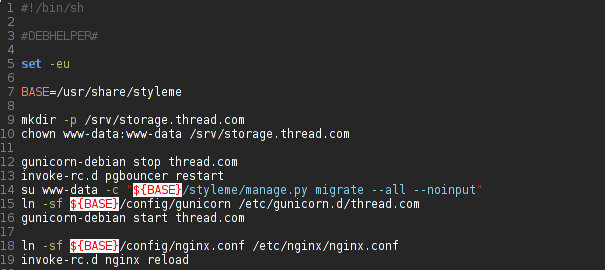
\includegraphics[width=100mm]{img/debian-postinst.png}
}


\frame {
    3/4: Auto-login links in emails
}

\frame {
    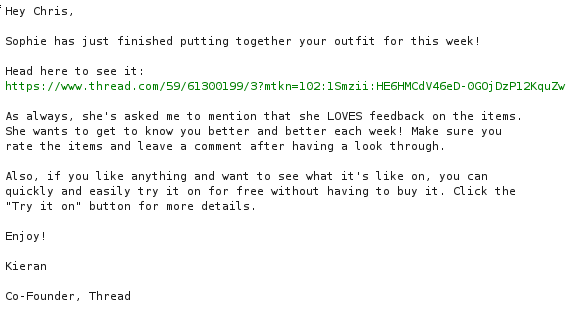
\includegraphics[width=100mm]{img/auto-login.png}
}

\frame {
    Our implementation

    \vskip 1em

    \begin{itemize}
        \item Allow login link to any URL
        \item Simple to use - can be added anywhere
        \item Salted HMAC implementation - no state
        \item Token includes timestamp so tokens expire
        \item Customisable salt fields - (default: {\tt User.password})
        \item Tokens can be re-used (feature)
        \item \url{https://github.com/playfire/django-autologin}
    \end{itemize}
}

\frame {
    Recommendations

    \vskip 1em

    \begin{itemize}
        \item Salt the HMAC with the user's hashed password
        \item Include the timestamp in the hash, not the expiry time
        \item Add "Click here to login" copy (aka "The forward problem")
    \end{itemize}
}

\frame {
    4/4: Git HEAD version of framework
}
 
\frame {
    \begin{itemize}
        \item Git HEAD of Django
        \item Updated approximately once a week via an embedded code copy
    \end{itemize}
}

\frame {
    Advantages

    \vskip 1em

    \begin{itemize}
        \item New features can save developer time
        \item Never complaining about missing features
        \item Security features often nice to have
        \item Increases incentive to send patches upstream
    \end{itemize}
}

\frame {
    Disdvantages

    \vskip 1em

    \begin{itemize}
        \item It breaks!
        \item 99\% of the time it breaks your libraries
    \end{itemize}

    \vskip 1em

    Nightmare mode: Git HEAD of your language runtime
}

\frame {}

\frame {
    fin
}

\end{document}
